

%% This file was auto-generated by IPython.
%% Conversion from the original notebook file:
%%
\documentclass[11pt,english]{article}

%% This is the automatic preamble used by IPython.  Note that it does *not*
%% include a documentclass declaration, that is added at runtime to the overall
%% document.

\usepackage{amsmath}
\usepackage{amssymb}
\usepackage{graphicx}
\usepackage{grffile}
\usepackage{ucs}
\usepackage[utf8x]{inputenc}

% Scale down larger images
\usepackage[export]{adjustbox}

%fancy verbatim
\usepackage{fancyvrb}
% needed for markdown enumerations to work
\usepackage{enumerate}

% Slightly bigger margins than the latex defaults
\usepackage{geometry}
\geometry{verbose,tmargin=3cm,bmargin=3cm,lmargin=2.5cm,rmargin=2.5cm}

% Define a few colors for use in code, links and cell shading
\usepackage{color}
\definecolor{orange}{cmyk}{0,0.4,0.8,0.2}
\definecolor{darkorange}{rgb}{.71,0.21,0.01}
\definecolor{darkgreen}{rgb}{.12,.54,.11}
\definecolor{myteal}{rgb}{.26, .44, .56}
\definecolor{gray}{gray}{0.45}
\definecolor{lightgray}{gray}{.95}
\definecolor{mediumgray}{gray}{.8}
\definecolor{inputbackground}{rgb}{.95, .95, .85}
\definecolor{outputbackground}{rgb}{.95, .95, .95}
\definecolor{traceback}{rgb}{1, .95, .95}

% new ansi colors
\definecolor{brown}{rgb}{0.54,0.27,0.07}
\definecolor{purple}{rgb}{0.5,0.0,0.5}
\definecolor{darkgray}{gray}{0.25}
\definecolor{lightred}{rgb}{1.0,0.39,0.28}
\definecolor{lightgreen}{rgb}{0.48,0.99,0.0}
\definecolor{lightblue}{rgb}{0.53,0.81,0.92}
\definecolor{lightpurple}{rgb}{0.87,0.63,0.87}
\definecolor{lightcyan}{rgb}{0.5,1.0,0.83}

% Framed environments for code cells (inputs, outputs, errors, ...).  The
% various uses of \unskip (or not) at the end were fine-tuned by hand, so don't
% randomly change them unless you're sure of the effect it will have.
\usepackage{framed}

% remove extraneous vertical space in boxes
\setlength\fboxsep{0pt}

% codecell is the whole input+output set of blocks that a Code cell can
% generate.

% TODO: unfortunately, it seems that using a framed codecell environment breaks
% the ability of the frames inside of it to be broken across pages.  This
% causes at least the problem of having lots of empty space at the bottom of
% pages as new frames are moved to the next page, and if a single frame is too
% long to fit on a page, will completely stop latex from compiling the
% document.  So unless we figure out a solution to this, we'll have to instead
% leave the codecell env. as empty.  I'm keeping the original codecell
% definition here (a thin vertical bar) for reference, in case we find a
% solution to the page break issue.

%% \newenvironment{codecell}{%
%%     \def\FrameCommand{\color{mediumgray} \vrule width 1pt \hspace{5pt}}%
%%    \MakeFramed{\vspace{-0.5em}}}
%%  {\unskip\endMakeFramed}

% For now, make this a no-op...
\newenvironment{codecell}{}

 \newenvironment{codeinput}{%
   \def\FrameCommand{\colorbox{inputbackground}}%
   \MakeFramed{\advance\hsize-\width \FrameRestore}}
 {\unskip\endMakeFramed}

\newenvironment{codeoutput}{%
   \def\FrameCommand{\colorbox{outputbackground}}%
   \vspace{-1.4em}
   \MakeFramed{\advance\hsize-\width \FrameRestore}}
 {\unskip\medskip\endMakeFramed}

\newenvironment{traceback}{%
   \def\FrameCommand{\colorbox{traceback}}%
   \MakeFramed{\advance\hsize-\width \FrameRestore}}
 {\endMakeFramed}

% Use and configure listings package for nicely formatted code
\usepackage{listingsutf8}
\lstset{
  language=python,
  inputencoding=utf8x,
  extendedchars=\true,
  aboveskip=\smallskipamount,
  belowskip=\smallskipamount,
  xleftmargin=2mm,
  breaklines=true,
  basicstyle=\small \ttfamily,
  showstringspaces=false,
  keywordstyle=\color{blue}\bfseries,
  commentstyle=\color{myteal},
  stringstyle=\color{darkgreen},
  identifierstyle=\color{darkorange},
  columns=fullflexible,  % tighter character kerning, like verb
}

% The hyperref package gives us a pdf with properly built
% internal navigation ('pdf bookmarks' for the table of contents,
% internal cross-reference links, web links for URLs, etc.)
\usepackage{hyperref}
\hypersetup{
  breaklinks=true,  % so long urls are correctly broken across lines
  colorlinks=true,
  urlcolor=blue,
  linkcolor=darkorange,
  citecolor=darkgreen,
  }

% hardcode size of all verbatim environments to be a bit smaller
\makeatletter 
\g@addto@macro\@verbatim\small\topsep=0.5em\partopsep=0pt
\makeatother 

% Prevent overflowing lines due to urls and other hard-to-break entities.
\sloppy




\begin{document}



\begin{codecell}


\begin{codeinput}
\begin{lstlisting}
#import filenames
import glob
no_strings_small =  glob.glob("no_strings_small/*.csv")
no_strings =  glob.glob("no_strings/*.csv")

all_strings = no_strings + no_strings_small

print all_strings

\end{lstlisting}
\end{codeinput}
\begin{codeoutput}


\begin{Verbatim}[commandchars=\\\{\}]
['no_strings/NoSurfaceObj_Pi-10.csv', 'no_strings/FiveSurfaceObj_PI-10.csv', 'no_strings/TwoSurfaceObj_PI-10.csv', 'no_strings_small/1_Object_PI-10.csv', 'no_strings_small/0_Object_PI-8.csv', 'no_strings_small/0_Object_PI-10.csv', 'no_strings_small/3_Object_PI-16.csv', 'no_strings_small/0_Object_PI-16.csv', 'no_strings_small/1_Object_PI-16.csv', 'no_strings_small/3_Object_PI-10.csv', 'no_strings_small/5_Object_PI-8.csv', 'no_strings_small/5_Object_PI-12.csv', 'no_strings_small/1_Object_PI-8.csv', 'no_strings_small/3_Object_PI-12.csv', 'no_strings_small/0_Object_PI-12.csv', 'no_strings_small/5_Object_PI-10.csv', 'no_strings_small/1_Object_PI-12.csv', 'no_strings_small/3_Object_PI-8.csv', 'no_strings_small/5_Object_PI-16.csv']
\end{Verbatim}

\end{codeoutput}

\end{codecell}

\begin{codecell}


\begin{codeinput}
\begin{lstlisting}
#read file
import csv
data = []

for s in [all_strings[0]]:
    f = open(s, "rb")
    names = csv.reader(f).next()
    rdr = csv.DictReader(f, fieldnames=names)

    data_part = [x for x in rdr]

    for d in data_part:
        for key in d:
            d[key] = float(d[key])
    data = data + data_part
    
print data[0]
#scatter([d['TestObjectX'] for d in data],
#        [d['TestObjectY'] for d in data],
#        c = [d['IsOnTheTable'] for d in data])
\end{lstlisting}
\end{codeinput}
\begin{codeoutput}


\begin{Verbatim}[commandchars=\\\{\}]
{'TestObjectX': -69.413742, 'TestObjectY': 22.394482, 'TestObjectZ': 0.600044, 'TestObjectHeight': 28.968426, 'TestObjectYaw': -86.811096, 'IsOnTheTable': 1.0, 'TestObjectWidth': 7.500002, 'TestObjectRoll': -0.616913, 'IsStatnding': 1.0, 'TestObjectLenght': 7.500001, 'TestObjectPitch': 3.938169}
\end{Verbatim}

\end{codeoutput}

\end{codecell}

\begin{codecell}


\begin{codeinput}
\begin{lstlisting}
#scatter data
import matplotlib.pyplot as plt
from mpl_toolkits.mplot3d import Axes3D

fig = plt.figure()
ax = fig.add_subplot(111, projection='3d')

plt.ion()

ax.scatter3D(
        [d['TestObjectX'] for d in data],
        [d['TestObjectY'] for d in data],
        [d['TestObjectZ'] for d in data],
        #[d['TestObjectRoll'] for d in data],
        #[d['TestObjectPitch'] for d in data],
        #[d['TestObjectYaw'] for d in data],
        c = [d['IsOnTheTable'] for d in data])
        #c = [d['IsStatnding'] for d in data])
   
\end{lstlisting}
\end{codeinput}
\begin{codeoutput}




\begin{verbatim}
<mpl_toolkits.mplot3d.art3d.Patch3DCollection at 0xd449ed0>
\end{verbatim}



\begin{center}
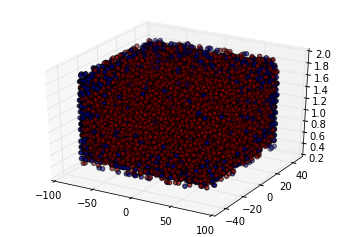
\includegraphics[max size={0.7\textwidth}{0.9\textheight}]{NN_ChristopheQuignon_050115_files/NN_ChristopheQuignon_050115_2_1.png}
\par
\end{center}

\end{codeoutput}

\end{codecell}

\begin{codecell}


\begin{codeinput}
\begin{lstlisting}
#train
from sklearn.svm import SVC

testdata = []
classification = []

for dset in data:
    setlist = []
    setlist.append(dset['TestObjectX'])
    setlist.append(dset['TestObjectY'])
    setlist.append(dset['TestObjectZ'])
    
    #setlist.append(dset['TestObjectRoll'])
    #setlist.append(dset['TestObjectPitch'])
    #setlist.append(dset['TestObjectYaw'])
    
    testdata.append(setlist)
    
    classification.append(dset['IsOnTheTable'])
    #classification.append(dset['IsStatnding'])
    
clf = SVC(
          C=1.00,
          kernel='rbf',#'rbf'
          #degree=60,
          gamma=0.20,
          #coef0=6.0,
          #shrinking=True,
          #probability=False,
          #tol=0.001,
          cache_size=2000,
          #class_weight=None,
          #verbose=False,
          #max_iter=-1,
          #random_state=None
          )

clf.fit(testdata, classification)


\end{lstlisting}
\end{codeinput}
\begin{codeoutput}




\begin{verbatim}
SVC(C=1.0, cache_size=2000, class_weight=None, coef0=0.0, degree=3, gamma=0.2,
  kernel='rbf', max_iter=-1, probability=False, random_state=None,
  shrinking=True, tol=0.001, verbose=False)
\end{verbatim}



\end{codeoutput}

\end{codecell}

\begin{codecell}


\begin{codeinput}
\begin{lstlisting}
#prepare range of random set
maxmin = []

maxmin.append([dset['TestObjectX'] for dset in data])
maxmin.append([dset['TestObjectY'] for dset in data])
maxmin.append([dset['TestObjectZ'] for dset in data])
#maxmin.append([dset['TestObjectRoll'] for dset in data])
#maxmin.append([dset['TestObjectPitch'] for dset in data])
#maxmin.append([dset['TestObjectYaw'] for dset in data])

for i in range(0, len(maxmin)):
    maxmin[i] = [min(maxmin[i]), max(maxmin[i])]

print maxmin
\end{lstlisting}
\end{codeinput}
\begin{codeoutput}


\begin{Verbatim}[commandchars=\\\{\}]
[[-80.0, 80.0], [-40.0, 40.0], [0.400032, 1.90004]]
\end{Verbatim}

\end{codeoutput}

\end{codecell}

\begin{codecell}


\begin{codeinput}
\begin{lstlisting}
#prediction on a random set
ps = []
preds = []

for _ in range(5000):
    p = []
    for d in maxmin:
        p.append(uniform(d[0], d[1]))
    ps.append(p)
preds = clf.predict(ps)

fig = plt.figure()
ax = fig.add_subplot(111, projection='3d')

plt.ion()

ax.scatter3D([p[0] for p in ps],
             [p[1] for p in ps],
             [p[2] for p in ps],
             #[p[3] for p in ps],
             #[p[4] for p in ps],
             #[p[5] for p in ps],
             c = preds)

\end{lstlisting}
\end{codeinput}
\begin{codeoutput}




\begin{verbatim}
<mpl_toolkits.mplot3d.art3d.Patch3DCollection at 0xd54b7d0>
\end{verbatim}



\begin{center}
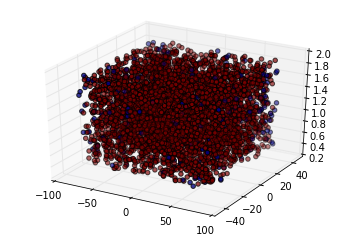
\includegraphics[max size={0.7\textwidth}{0.9\textheight}]{NN_ChristopheQuignon_050115_files/NN_ChristopheQuignon_050115_5_1.png}
\par
\end{center}

\end{codeoutput}

\end{codecell}

\begin{codecell}


\begin{codeinput}
\begin{lstlisting}
print preds
print sum(preds)/len(preds)
#well, that's optimistic
\end{lstlisting}
\end{codeinput}
\begin{codeoutput}


\begin{Verbatim}[commandchars=\\\{\}]
[ 1.  1.  1. ...,  1.  1.  1.]
0.9476
\end{Verbatim}

\end{codeoutput}

\end{codecell}

\begin{codecell}


\begin{codeinput}
\begin{lstlisting}
print sum(classification)/len(classification)
\end{lstlisting}
\end{codeinput}
\begin{codeoutput}


\begin{Verbatim}[commandchars=\\\{\}]
0.90998
\end{Verbatim}

\end{codeoutput}

\end{codecell}

\begin{codecell}


\begin{codeinput}
\begin{lstlisting}
#Validation with the same set
preds = clf.predict(testdata)

fig = plt.figure()
ax = fig.add_subplot(111, projection='3d')

plt.ion()

ax.scatter3D([d[0] for d in testdata],
             [d[1] for d in testdata],
             [d[2] for d in testdata],
             c = preds)

\end{lstlisting}
\end{codeinput}
\begin{codeoutput}




\begin{verbatim}
<mpl_toolkits.mplot3d.art3d.Patch3DCollection at 0xc91f890>
\end{verbatim}



\begin{center}
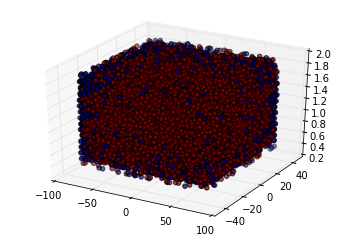
\includegraphics[max size={0.7\textwidth}{0.9\textheight}]{NN_ChristopheQuignon_050115_files/NN_ChristopheQuignon_050115_8_1.png}
\par
\end{center}

\end{codeoutput}

\end{codecell}

\begin{codecell}


\begin{codeinput}
\begin{lstlisting}

\end{lstlisting}
\end{codeinput}

\end{codecell}



\end{document}

